 \chapter {基于Wi-Fi信号的手势被动感知技术}

 \section{引言}

\subsection{Wi-Fi信号与感知}

Wi-Fi是一种基于802.11协议标准的无线局域网技术。802.11协议的原始标准最早出现在1997年, 近十几年其标准也在随着新技术的出现不断演进。从Wi-Fi的设计意图和实际的应用情况看,它似乎只是一种适用于无线局域网的通信方式。然而随着支持Wi-Fi的设备越来越普及,科研人员一直在寻求基于Wi-Fi的新应用,例如,开发Wi-Fi信号的感知能力。


随着Wi-Fi物理层能力的提升,重用Wi-Fi通信信号进行无线感知成为可能\upcite{lvwirelesssurvey}。Wi-Fi的角色正在从一个单纯的通信工具到一个感知平台进行演化。在室内,传播环境会影响信号传播状态,Wi-Fi发出的信号会经过直射,环境的反射或者散射,最终到达接收端。即接收端收到的信号中其实除了数据还包括环境信息。只需找到合适的方法,就可将其中包含的环境信息提取出来\upcite{wu2016widir,wang2016human,wang2016gait}。这里的环境信息主要指两个方面:外部物体(墙体、障碍物)和人(人的位置,人的姿势等)。

用无线信号感知环境信息并不是一个新鲜的想法。早在二战时期,人们便开始使用基于无线电的物体感知系统,即雷达\upcite{barton1988modern}。雷达主要应用在室外,通过分析物体反射回来的无线点信号,不仅可以得到物体类型、距离范围,还可以推算物体运动距离。近几年人们还研发了可以应用于室内的超宽带雷达系统。但这两种应用都需要专用信号,且需昂贵的专业设备的支持,不适合大规模民用。

%\subsection{相关工作}

人们对智能生活的想象力在不断丰富。适合于室内的物体感知和定位技术成为了研究人员的新方向。例如,基于被动感知的人员检测。被检测着不需要携带任何设备,检测设备通过无线信号的变化推测出是否有人出现。这一技术可以广泛应用到安防设备和智能家居中,以提供无缝的交互体验。另一个例子是室内定位,虽然基于GPS的定位精度已经很高,但室内无法接收GPS信号。相反,现今大型商场中随处可以Wi-Fi信号。因此近两年来基于Wi-Fi的室内定位技术十分火热,技术也日趋成熟,识别精度令人惊艳。相信很快基于Wi-Fi的室内定位技术就可以应用到实际产品中,手机用户再也不会因为室内接受不到GPS信号而在大型商场中迷路。

人机交互是智能生活的重要组成部分。计算机发展之处,键盘鼠标可以说代表了一种先进的技术,然而现在它们已经过时了。基于无设备接触的语音、和手势才是和智能设备交互的趋势。语音交互方面的研究,国内的科大讯飞首屈一指,识别正确率高达97\%,每分钟可识别400字。而手势识别相关技术还存在很多问题。手势识别相关研究百花齐放,除了现有基于摄像头的成型产品,还有基于红外线的、基于声音的、基于穿戴设备的相关研究。而本章将研究另外一种手势识别的实现方式,即基于Wi-Fi信号。

%信号的传播环境会直接影响接收端的信号质量,CSI描述的正是接收端的信号质量。

 \subsection{基于Wi-Fi信号感知的优势及困难}

基于Wi-Fi感知手势主要存在以下几点优势:1)Wi-Fi信号的传播是超视距的\upcite{chang2016we},即使手势与设备间存在障碍物,甚至有一面墙,也不会影响识别效果。相对来说,基于摄像头和红外线的手势识别则只能工作在视距范围内。对于摄像头来说,它还会收到光线的影响。2)无需部署额外设备。相比于基于穿戴设备的手势识别,一方面用户不用付出额外的硬件成本。另一方面,用户也不用在为必须要携带额外的随身设备而困扰,毕竟现代人已经有够多的电子设备需要充电。实际上,该项技术几乎是零成本的,现今智能设备普遍配有Wi-Fi,这里只是对Wi-Fi的一种重用。

无线信号感知手势存在优势,也存在困难。1)Wi-Fi信号本身也存在自己的不稳定,一则由于内部电流的不稳定,二则环境中也存在不可控的微小变化。因此在研究中,消除干扰是必须解决的困难。2)不同于基于摄像头的手势识别,可以将成熟的图像建模技术应用其中。基于Wi-Fi信号的手势识别目前并没有成熟信号建模技术。如何从变化的信号中提取出手势信息还有待探索。


\subsection{从信号强度到信道状态信息}

无线信号的感知是基于其底层的传播特性\upcite{yang2013rssi,pu2013whole,ding2016device}。信号强度(Received Signal Strength Indicator,RSSI)就可以用做感知。一个较强的RSSI表示较短的传播距离,反之则代表两个设备间距离较远。可以说在过去的二十年基于信号强度的感知应用在快速发展,已经成为无线感知的典型代表。

RSSI可以大致反映无线信号的传输距离,但不够可靠。这里的信号不仅包含Wi-Fi,还包含蓝牙、RFID、GSM和WCDMA等3G或4G技术。智能手机在不开启GPS的情况下,如果使用LBS服务,其定位技术就是依靠手机信号的RSSI估算传输距离来实现。然而RSSI除了和传输距离有关还会受多径效应影响,所以在基站密度高,障碍物较少的情况下,才能达到较高的定位精度。而当传播环境差,多径效应明显时,定位精度差强人意。

Wi-Fi的RSSI同样存在受多径影响的问题。普通家庭环境中,Wi-Fi热点个数少,障碍物多,多径效应明显。经研究表明,即使在热点和信号接收设备都保持静态的情况下,RSSI也在不停变化,且变化幅度高达5分贝。这样的RSSI用在室内定位技术上尚且不够稳定,用来进行手势识别更是无从谈起。

相对于MAC层的RSSI,物理层的CSI可以提供更详细的信息\upcite{qian2014usrpsensing}。多径传播可以用信道冲击响应(Channel Impulse Response,CIR)来描述。在时不变的假设下,CIR可以公式~\ref{equ:cir}所示模型表示。
\begin{equation}
\label{equ:cir}
h\left( t \right) = \sum\limits_{i = 1}^N {{a_i}} {e^{ - j{\theta _i}}}\delta \left( {\tau  - {\tau _i}} \right)
\end{equation}

公式~\ref{equ:cir}中,$a_i$,$\theta _i$和$\tau _i$分别表示信号的幅值,相位以及第$i$个路径上的延时。$N$表示路径个数,$\delta \left( \tau \right)$表示狄克拉函数。每一个脉冲代表了一个传播路径。相位的叠加会导致其增强或抵消,表现出频率选择性衰减。因此可以通过信道频率响应Channel Frequency Response,CFR)来刻画多径效应,CFR正是CIR做傅里叶变换以后的结果。

想要获取较精确的CIR或者CFR一般需要使用昂贵的探测仪。然而比较幸运的是基于OFDM技术的Wi-Fi设备已经在其底层提供了子载波级别的CFR信息。对商业Wi-Fi,只需对固件驱动做相应修改,底层便可以CSI的形式返回我们需要的信息。

CSI提供的信息要比RSSI更加精细。如果说RSSI是一束光,那么CSI可以看作是这束光里包含的赤橙黄绿等颜色的具体信息。当人手在环境中挥动时,RSSI可能无法感知到环境中的变化,但CSI可以感知到。

\section{系统设计与实现}
\subsection{系统架构}
基于Wi-Fi的手势感知系统大致可以分为CSI数据的获取、CSI数据的处理与分析和CSI数据的可视化三个模块。如图~\ref{fig:wisenseArc}所示,CSI获取数据后将数据同时传递给数据处理与分析模块和可视化模块。上层的两个模块处于并行的关系,互不影响。

\begin{figure}[htbp] % use float package if you want it here
  \centering
  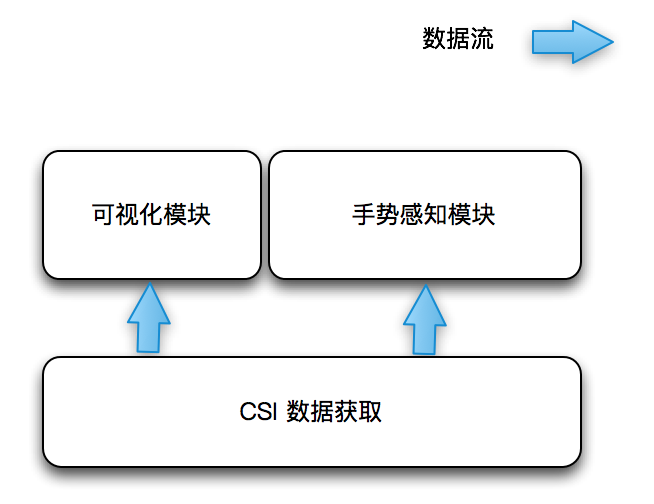
\includegraphics[width=3in]{wisenseArc}
  \caption[Wi-Fi手势感知系统架构]{Wi-Fi手势感知系统架构}
  \label{fig:wisenseArc}
\end{figure}

\subsection{环境设置与手势设计}
\subsubsection{环境设置}

已有利用Wi-Fi信号做感知的研究中,研究者多是在某一个固定环境下收集样本数据。利用这些样本数据训练模型,并在相同环境下测试模型效果。然而,事实上,无论是基于Wi-Fi信号RSSI还是CSI做感知,环境的影响都是不可忽略的一环。因此本文选择将环境变量纳入研究。

实验环境设置在一个具有两个房间的环境中,如图~\ref{fig:enviroment}所示。实验者共布置了两台设备。一台发送信号的设备,固定位置。一台接收信号的设备,根据实验需要在两个房间切换。一个障碍物,具体位置根据实验需求摆放。实验者在接收端、中间或发送端做手势,具体位置如图~\ref{fig:locations}所示。

\begin{figure}[htbp] % use float package if you want it here
  \centering
  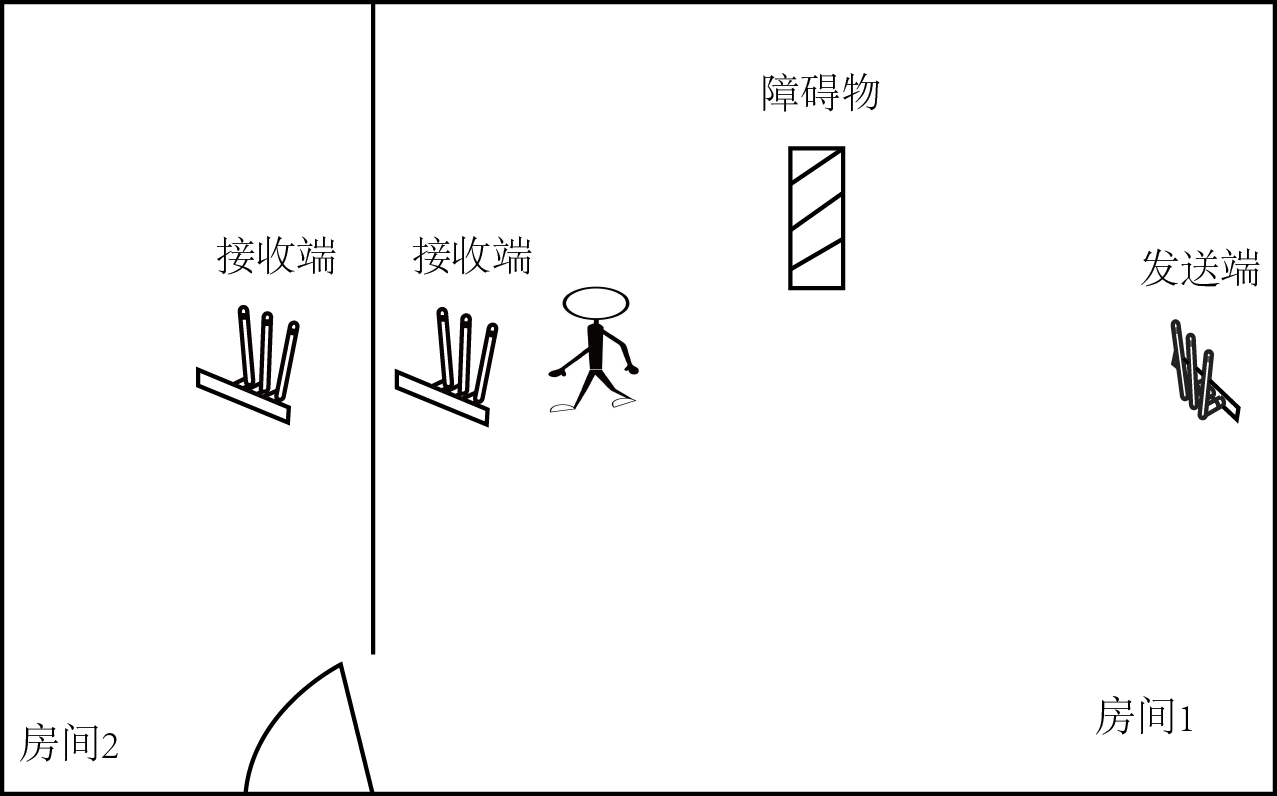
\includegraphics[width=3in]{environment}
  \caption{数据采集环境}
  \label{fig:environment}
\end{figure}

\begin{figure}[htbp] % use float package if you want it here
  \centering
  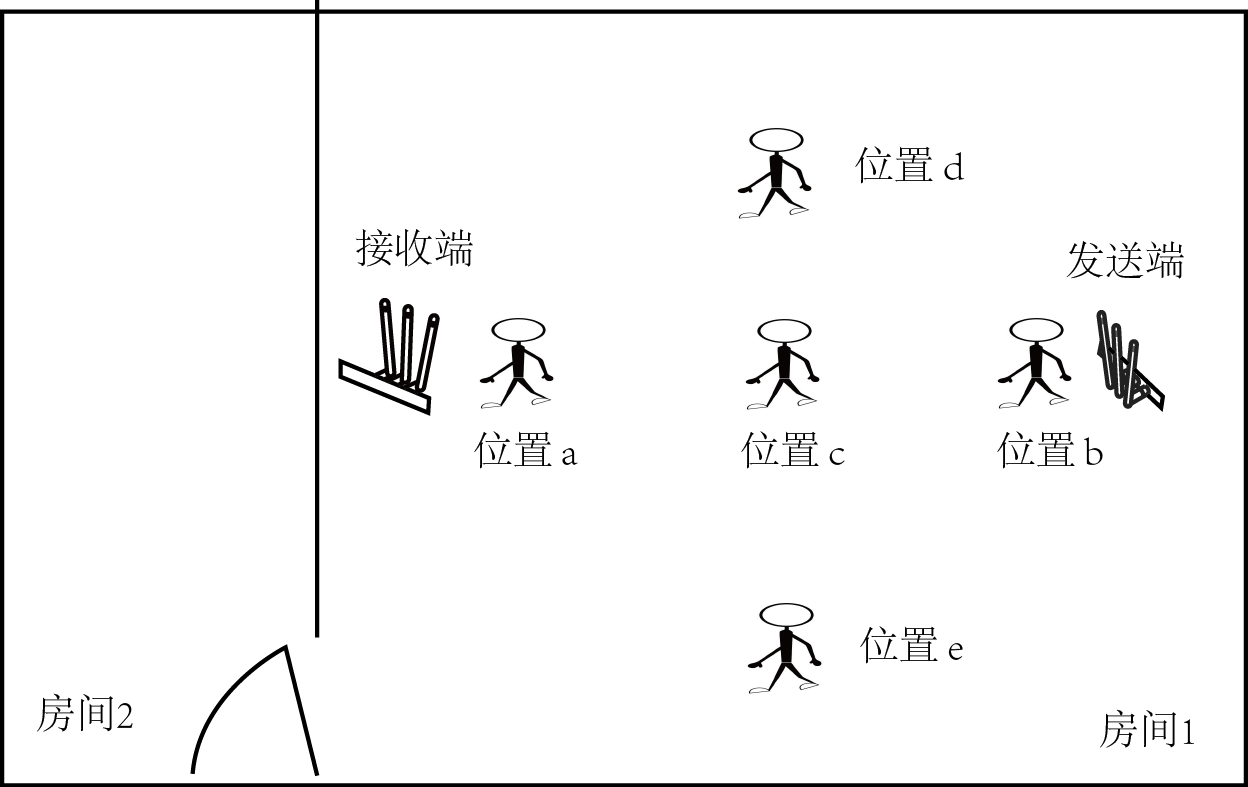
\includegraphics[width=3in]{locations}
  \caption{实验者位置}
  \label{fig:locations}
\end{figure}
% \begin{figure}[htbp] % use float package if you want it here
% \begin{minipage}{0.48\textwidth}
%   \centering
%   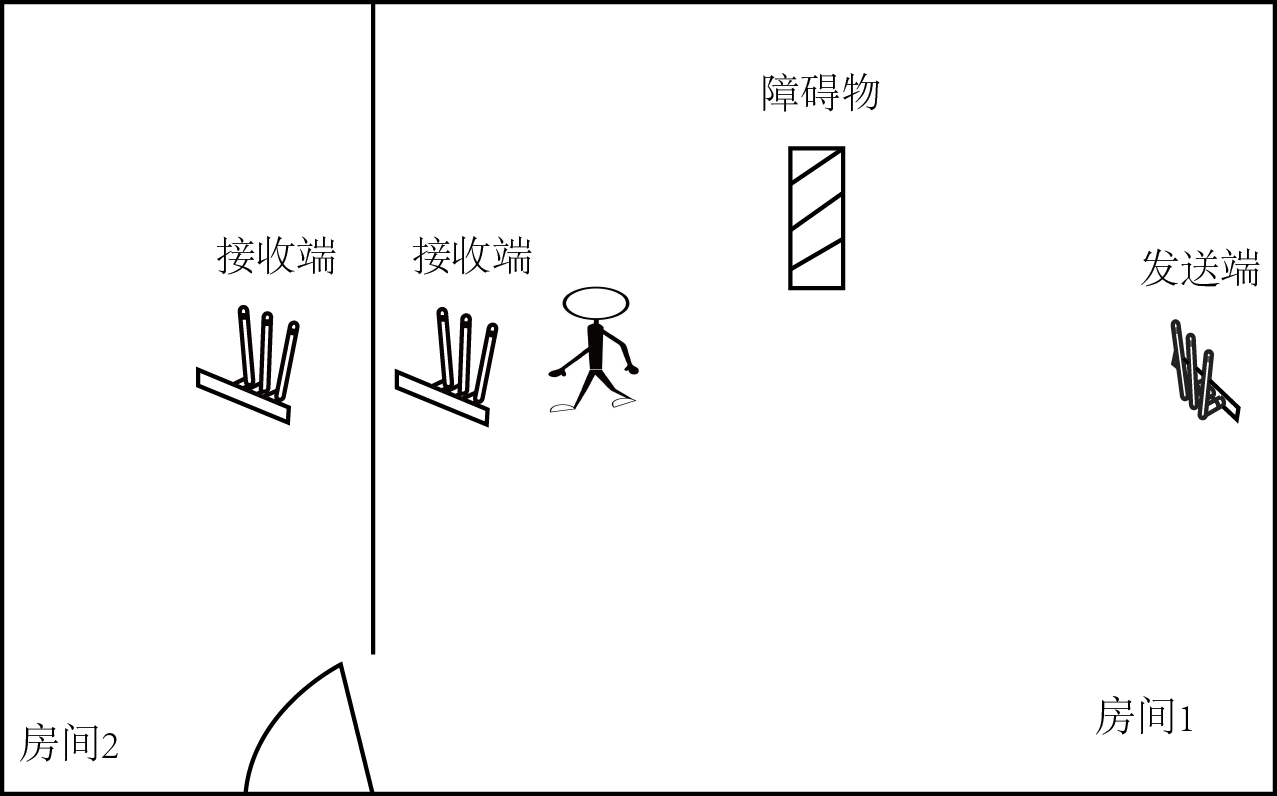
\includegraphics[width=3in]{environment}
%   \caption{数据采集环境}
%   \label{fig:environment}
% \end{minipage}\hfill
% \begin{minipage}{0.48\textwidth}
%   \centering
%   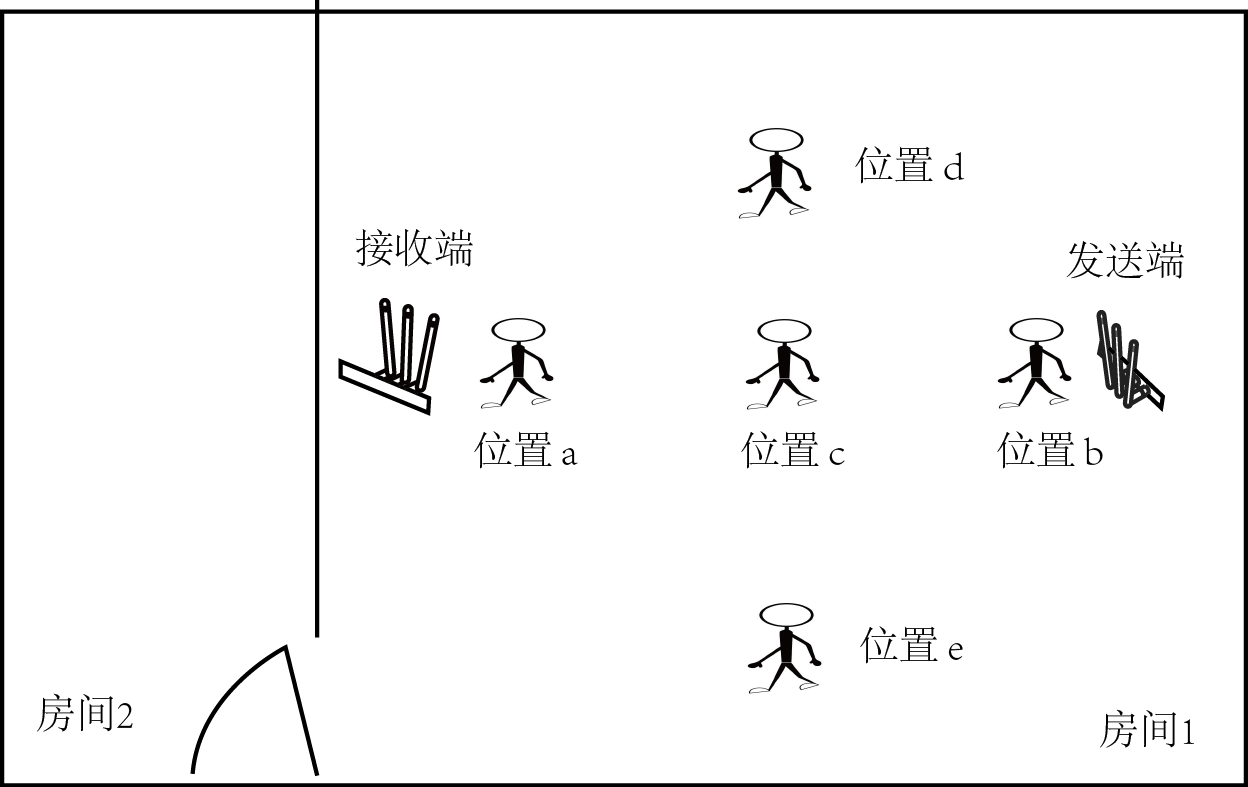
\includegraphics[width=3in]{locations}
%   \caption{实验者位置}
%   \label{fig:locations}
% \end{minipage}
% \end{figure}



\subsubsection{手势设计}

考虑到手势对CSI的影响可能源自手势路径,手势方向,手势切入方式等方面,本文采集了五种手势的样本进行训练与分析。这五种手势的具体动作如图~\ref{fig:actions}所示。

\begin{figure}[htbp] % use float package if you want it here
  \centering
  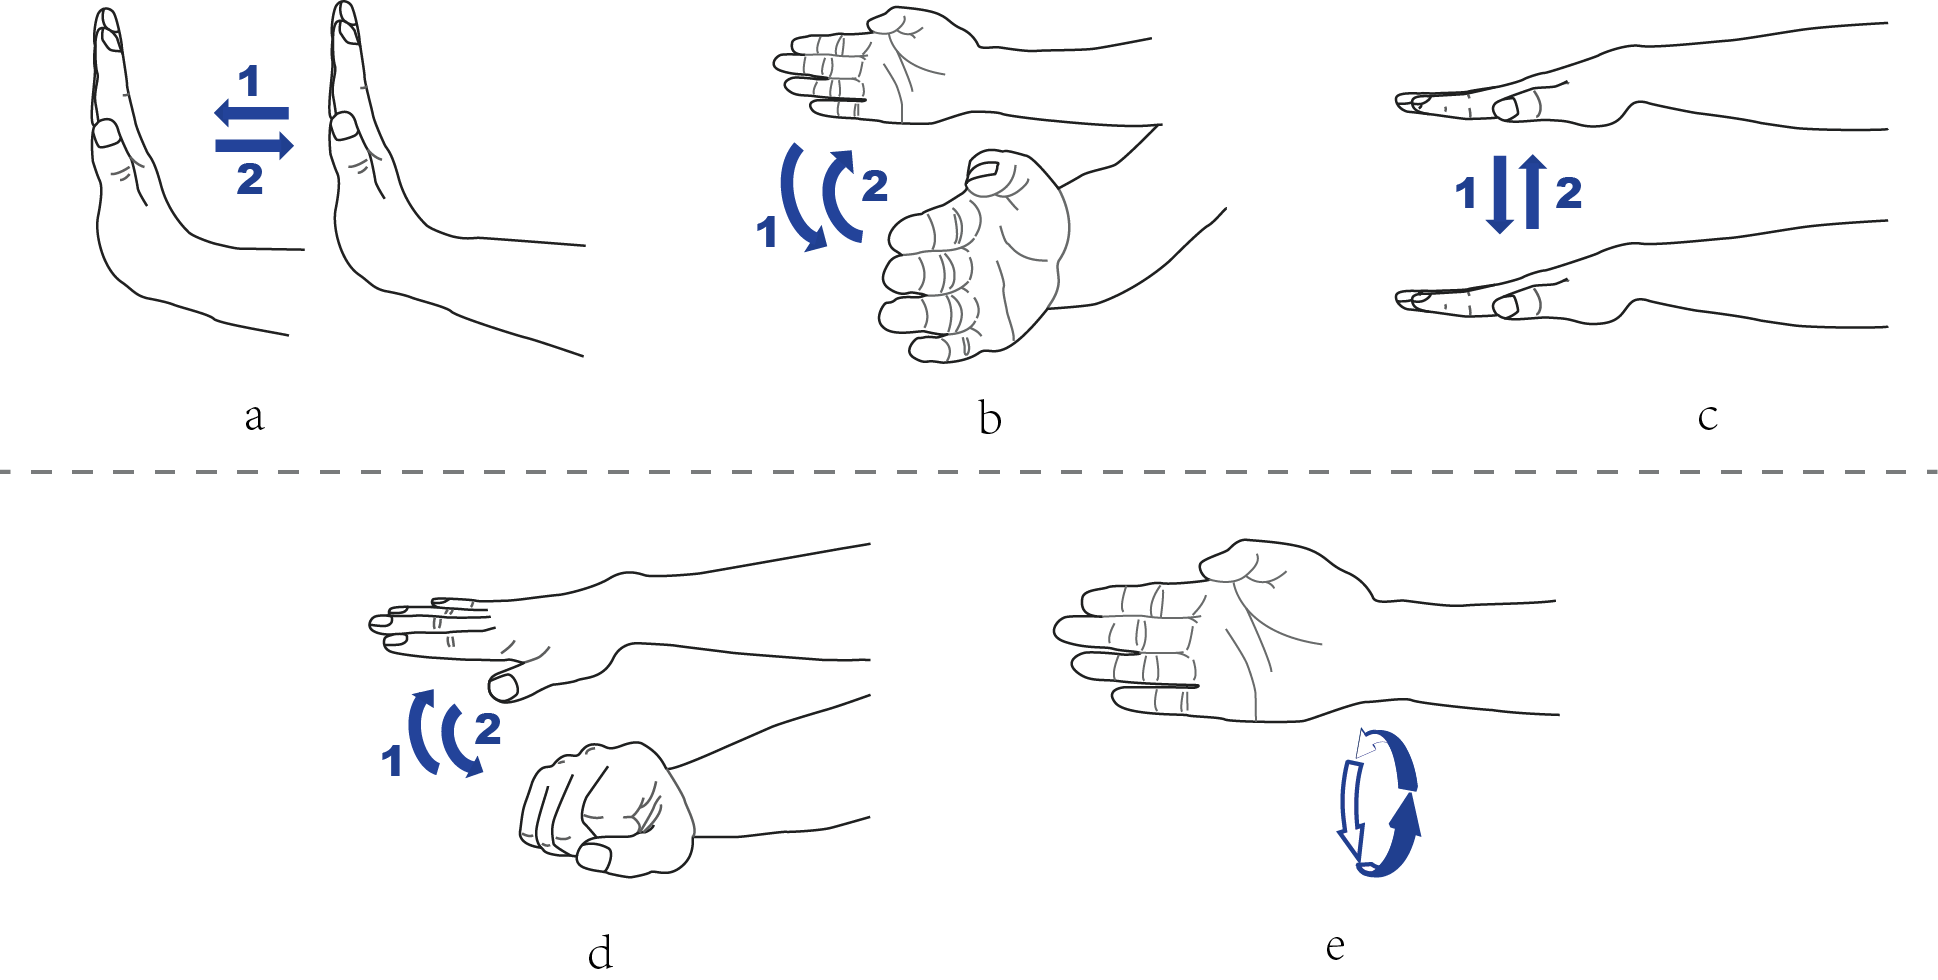
\includegraphics[width=6in]{actions}
  \caption{五种手势动作}
  \label{fig:actions}
\end{figure}

 \subsection{CSI数据的获取}
信道状态信息(Channel State Infomation,CSI)是一组可以反映信号传播路径的物理层信息。普通商用Wi-Fi并没有向用户提供信道状态信息,但是可以通过修改网卡驱动的方式获取。

 \subsubsection{定制内核驱动}
CSI属于物理层信息,获取CSI的一种方式是利用软件无线电设备(USRP),但其设备昂贵,不具有普适性。另一种方式基于开源的网卡驱动代码定制网卡驱动。本文的研究是基于定制驱动的方式实现。由于需要有开源驱动代码的支持,网卡型号的选择十分受限,本研究选择的是基于Atheros AR938x芯片的TP-link三天线网卡,并在前人的工作上做了适配。

经过多方面的对比,本文选择基于新加坡南洋理工的研究员发布的Atheros CSI工具进行适配。该工具可以帮助我们从物理层提取CSI、RSSI、时间戳、数据载荷等多方面信息。在获取的数据方面也有多方面优势:

\begin{compactenum}
\item 无分组无压缩的CSI数据。无分组是指其返回的CSI数据中包含了每个子载波的单独信息,即20MHz的信道有56个子载波,40MHz的信道有114个子载波。无压缩是指其返回的数据包含有足够的精度,即分别用10个比特位表示实部和虚部。
\item 详细的载荷数据。可以记录每一个包的载荷内容,包括接受到的数据包有哪些错误的比特位,以及导致这些错误的原因。
\item 丰富的信息。除了可以提供CSI外,还可以提供信道主频、时间戳、带宽、子载波数量和传输错误类型等信息。
\item 支持广播模式。方便同时在多个地点部署CSI接收端。如图~\ref{fig:Broadcast}所示。
\begin{figure}[htbp] % use float package if you want it here
  \centering
  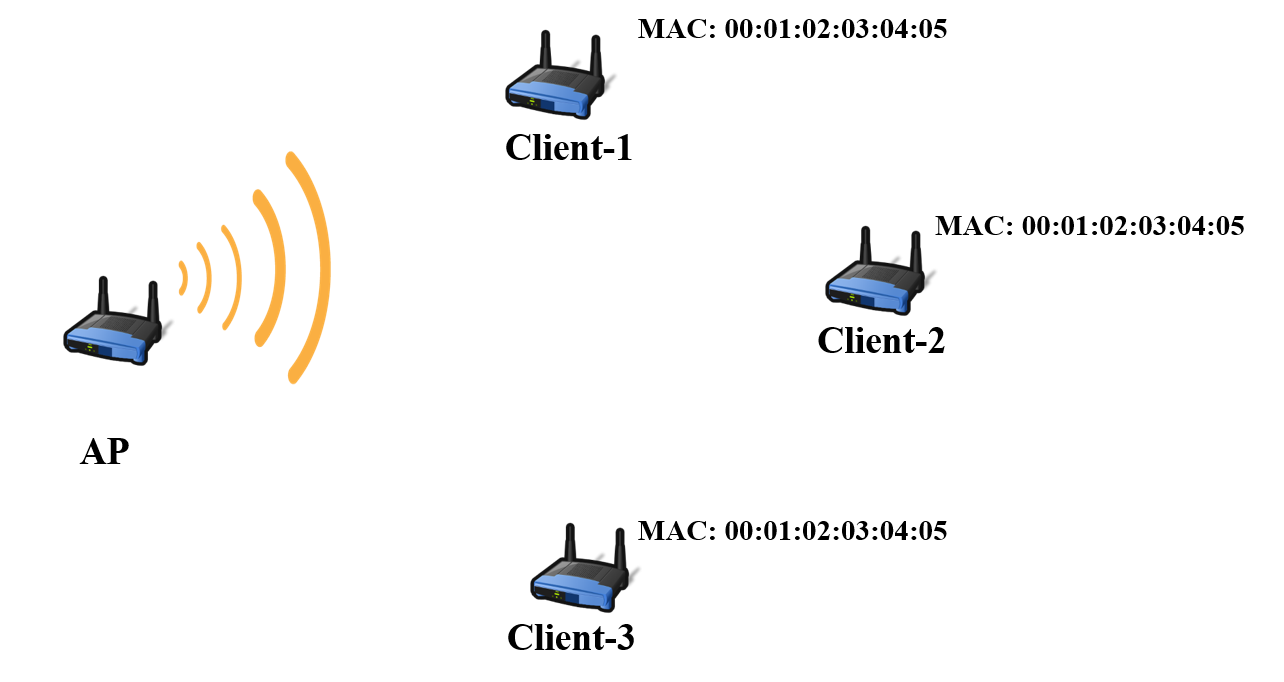
\includegraphics[width=3in]{Broadcast}
  \caption{广播模式}
  \label{fig:Broadcast}
\end{figure}
\end{compactenum}

在两台主机上配置好定制的网卡内核驱动后,将发送端设置为热点模式,假设一个Wi-Fi热点,接收端主动连接上相应Wi-Fi热点。当有数据在链路中传输时,就会有CSI信息从内核层传递到应用层。接收端和发送端都可以读取。

获取到的CSI信息举例:
\begin{code}[numbers=none]
 csi = 
 timestamp: 1477316861
 csi_len: 420
 channel: 2442
 err_info: 0
 noise_floor: 0
 Rate: 133
 bandWidth: 0
 num_tones: 56
 nr: 3
 nc: 1
 rssi: 56
 rssi1: 47
 rssi2: 458
 rssi3: 57
 payload_len: 1040
 csi: [3x1x56 complex double]
 payload: [1040x1 uint8]
 \end{code}

\subsection{数据可视化}
%(感知过程需要对数据实时处理,可视化是为了方便研究观察)

为了更好的观察CSI随环境及手势的变化,我们以时间为横轴,振幅为纵轴绘制了CSI的实时波形图。其中,数据读取进程采用C语言实现。图形绘制则使用脚本语言Python编写,调用matplotlib图形库。数据读取与图形绘制两进程间使用socket通信。可视化结果如图~\ref{fig:csi_plot}所示。

\begin{figure}[htbp] % use float package if you want it here
  \centering
  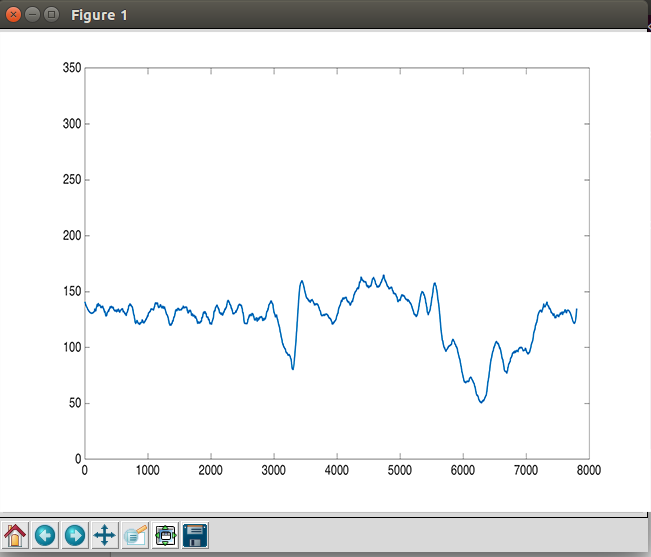
\includegraphics[width=3in]{csi_plot}
  \caption{CSI波形可视化}
  \label{fig:csi_plot}
\end{figure}

\section{手势感知模型}

\subsection{CSI数据变化分析}
CSI反映的是信号的传播质量,它除了受接收端与发送端的距离影响外,还受多径效应的影响。信号传播环境的变化会直接影响造成信号多径效应的反射、散射或是直射情况,最终会反映到CSI的变化上来。
\subsubsection{环境对信号传播路径的影响}
普通商用Wi-Fi的天线多为全向天线。全向天线的信号就像灯光一样向四周发散开,一部分信号直射到视距范围内的接收端,一部分信号会撞到障碍物(人、墙、普通障碍物)然后经过各种反射、散射,最终到达接收端。因此当信号传播路径中的障碍物布局发生了变化,其对应位置的信号就会受影响。如图~\ref{fig:signalAffected}所示,假设从发送端到接收端存在4条传播路径,一条直射路径,三条反射路径。当一个人作为障碍物出现在图中位置时,图示中的两条反射路径就会随之受影响,但另外一条反射路径和直射路径保持不变。


\begin{figure}[htbp] % use float package if you want it here
  \centering
  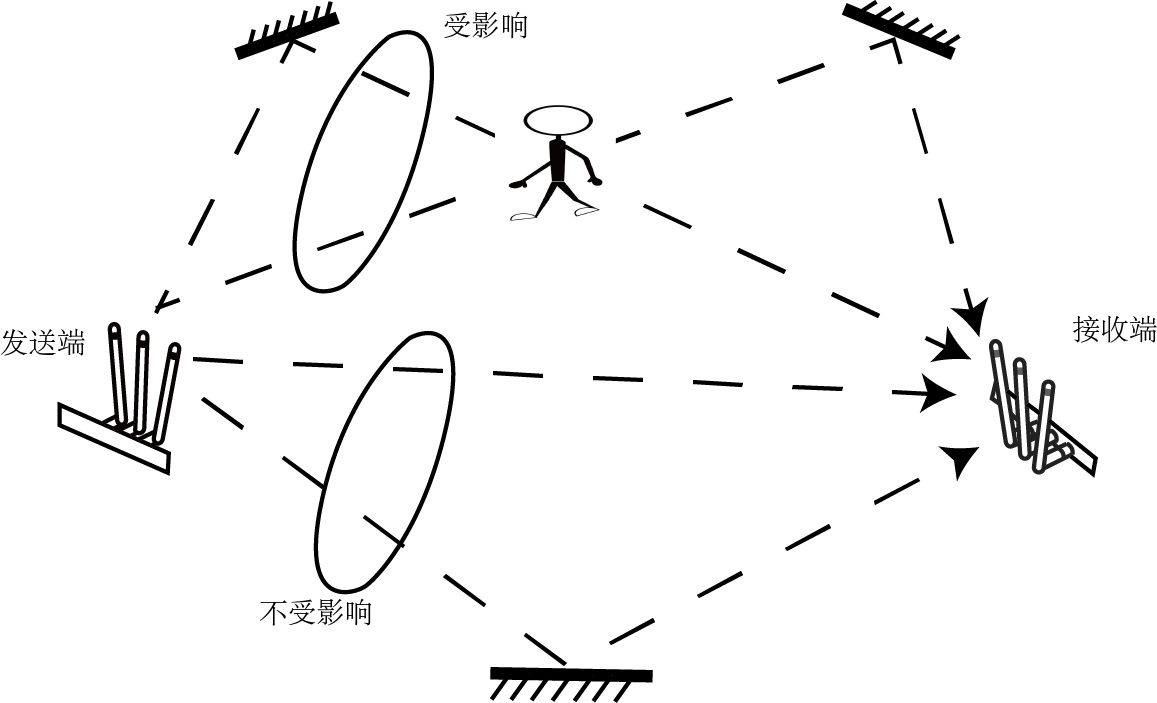
\includegraphics[width=3in]{signalAffected}
  \caption{障碍物对信号传播路径的影响}
  \label{fig:signalAffected}
\end{figure}

\subsubsection{环境对CSI幅值的影响}
上文分析了环境变化对信号传播路径的影响,其造成的影响最终会反映到CSI数据中。为了探究环境与CSI的关系,我们设计了多组实验。实验考虑了人、墙、普通障碍物三种因素设计了四组对比实验:不同的人遮挡,同一个人在不同位置遮挡,有无物体障碍物和是否穿墙。每种环境下收集了二十组数据,将二十组数据求平均并随机采样绘制对比图。其结果如图~\ref{fig:scatterfig}所示。
\begin{figure}[htbp] % use float package if you want it here
  \centering
  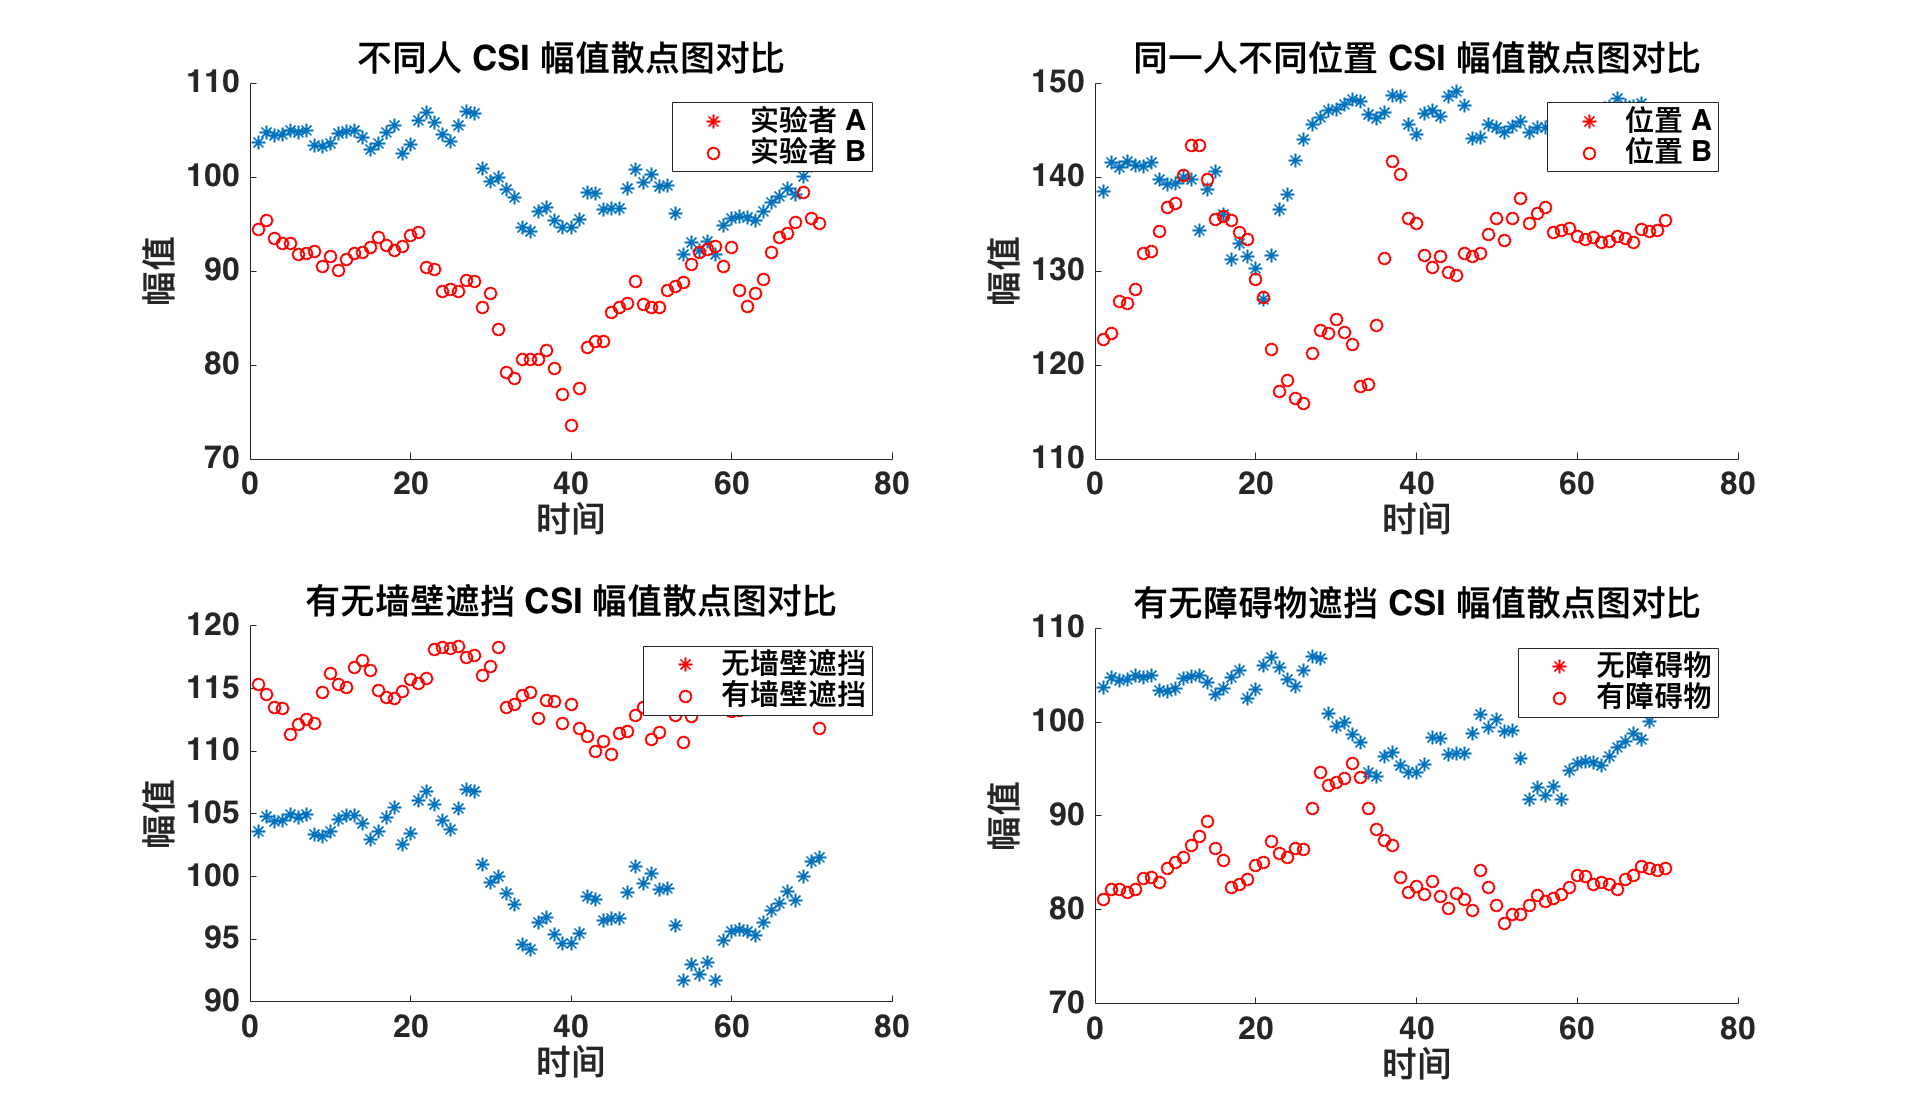
\includegraphics[width=6in]{scatterfig}
  \caption{环境对CSI幅值的影响}
  \label{fig:scatterfig}
\end{figure}

图~\ref{fig:scatterfig}表明:不同人站在同一位置对信号传播主路径进行遮挡效果有较大差别;同一个人站在不同位置的遮挡对CSI的影响有差别;有无墙的遮挡对CSI影响很大,但由于设备自动调节功率的功能,当接收设备穿墙后发送端随之增大发射功率,导致出现穿墙时CSI幅值更高的情况;有无障碍物对CSI亦有一定影响,但没有达到促使发送端增大功率的强度。

\subsubsection{不同样本间的相关性分析}
用Wi-Fi信号的CSI识别手势的一个基本假设是:不同手势对CSI的影响不同,相同手势对CSI的影响相似。这里将通过实验对基本假设进行验证。实验采用单一变量法,固定除手势外其它环境因素,接收端和发送端之间没有墙面遮挡(环境A)采集两组数据,每组数据二十个样本。第一组,实验员在信号传播的主路径做图~\ref{fig:actions}中的手势一;第二组,实验员在信号主路径做图中的手势二。我们分析了第一组数据间的自相关性,第二组数据间的自相关性以及第一组数据与第二组数据之间的互相关性,结果如图~\ref{fig:corrfig_1}所示。

\begin{figure}[htbp] % use float package if you want it here
  \centering
  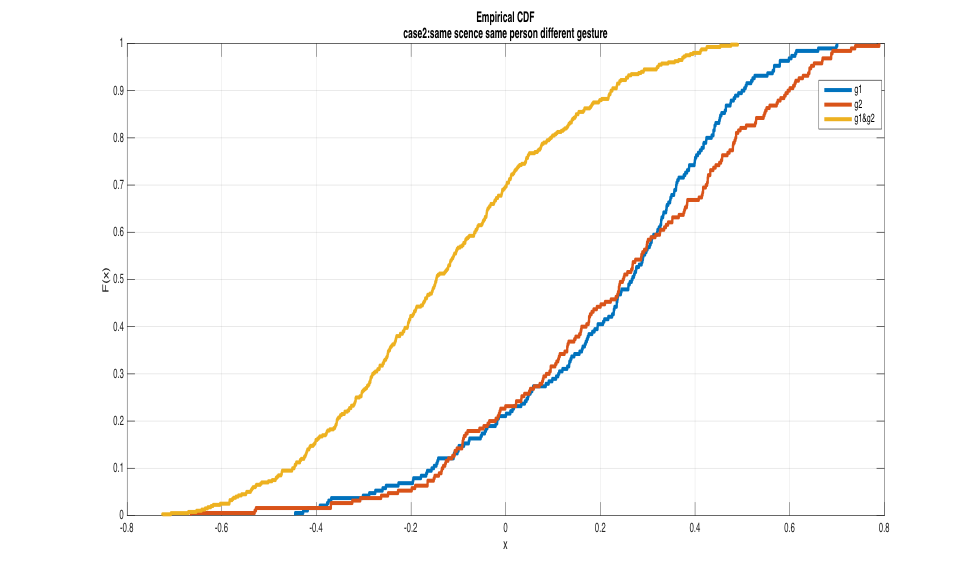
\includegraphics[width=3in]{corrfig_1}
  \caption{环境对CSI幅值的影响}
  \label{fig:corrfig_1}
\end{figure}

从图~\ref{fig:corrfig_1}中可以看出,代表相同手势的CSI数据间相关性在0.2以上的中有60\%。与之相对的,代表不同手势的CSI数据间的相关性有90\%是小于0.2的。该结果从侧面向我们证实了基本假设,即相同手势对CSI造成的影响相似,不同手势对CSI造成的影响差异大。

实际应用中,除手势外的信号传播环境不可能一成不变,因此要想成功识别手势还需要另一个假设成立:同一手势在不同环境下样本间距离要小于不同手势样本间距离,具体如图~\ref{fig:corrfig_2}所示。该假设成立才能保证手势识别的工作对环境具有一定鲁棒性。

\begin{figure}[htbp]
\centering
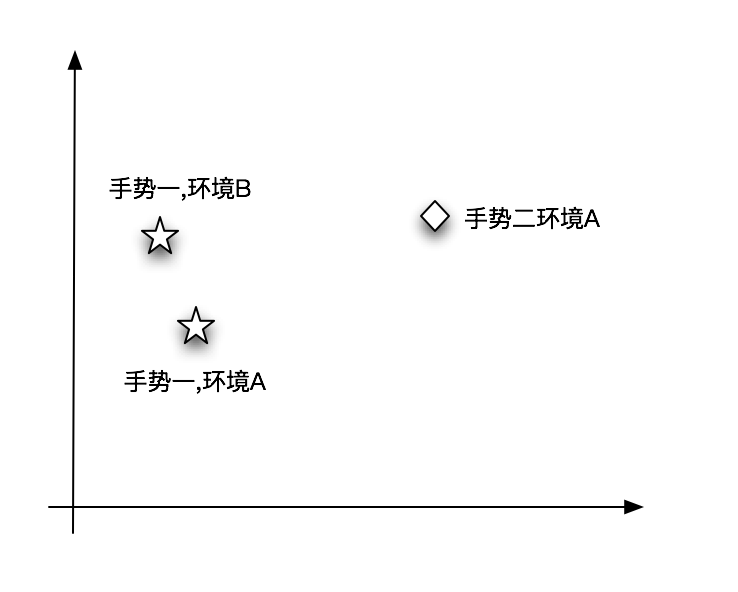
\includegraphics[width=3in]{corrfig_2}
\caption{手势识别对环境的鲁棒性假设}
\label{fig:corrfig_2}
\end{figure}

下面增加一组实验从侧面验证以上假设。增加的实验为实验员在穿墙环境(环境B)下做手势一,同样采集20个样本。计算相关性,绘制分布图,结果如图~\ref{fig:corrfig_3}所示。从图中可以看出,环境A中手势一的样本间相关性最强,环境A中手势一与环境A中手势二的样本间相关性最差,环境A中手势一与环境B中手势一的相关分布曲线介于另外两条曲线之间,且没有交叉。结果从侧面反映了手势识别对环境的改变具有一定容忍性。

\begin{figure}[htbp] % use float package if you want it here
  \centering
  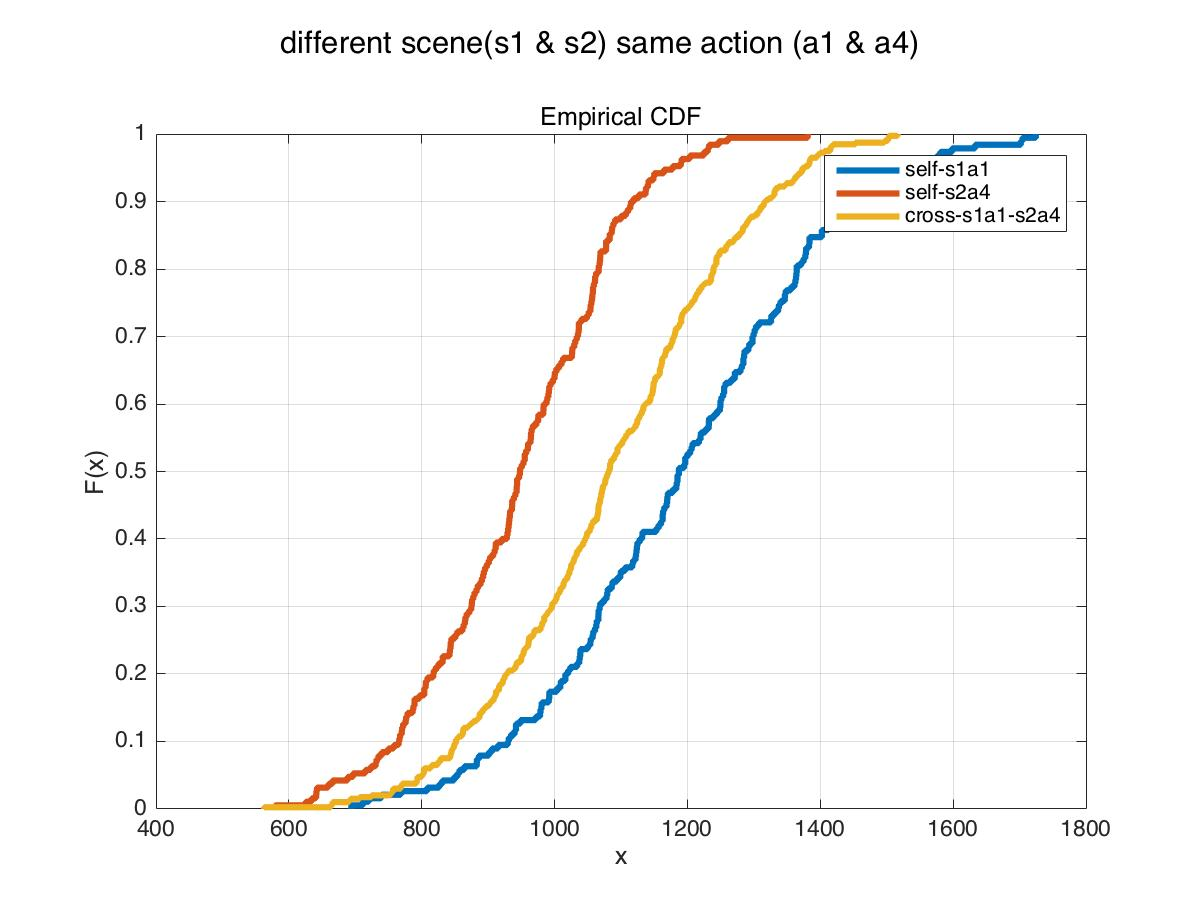
\includegraphics[width=3in]{corrfig_3}
  \caption{手势识别对环境的鲁棒性验证}
  \label{fig:corrfig_3}
\end{figure}

\subsubsection{同样本不同子载波间的相关性分析}

随着OFDM技术的出现,多天线设备开始流行,本研究中所用网卡即是支持OFDM的三根天线设备。在OFDM中一个信道被分为56或114个相互叠加的子载波,子载波间并行或串行的传输数据。运行OFDM协议的三天线设备CSI信息实际上是一个$3 \times 3 \times 56$的矩阵,其中第一维度对应接收端的三根天线,第二维度对应发送端三根天线,第三维度则对应56个子载波。加上时间维度,总共可以得到$3 \times 3 \times 56$条时间-幅度曲线。结果大量实验与分析我们发现这504组数据存在一定的关联。当信号传播环境保持不变时,代表不同子载波的CSI波形呈现随机性,无序性,无明显关联;当信号传播环境发生规律性的改变时(例如,有人在做指定手势)和同一天线有关的子载波开始变的相关,如图~\ref{fig:corrfig_4}所示。我们认为,这是由于环境变化对各子载波造成的影响相似,各子载波对应的CSI变化也就呈现除了大体上的相似性。

\begin{figure}[htbp] % use float package if you want it here
  \centering
  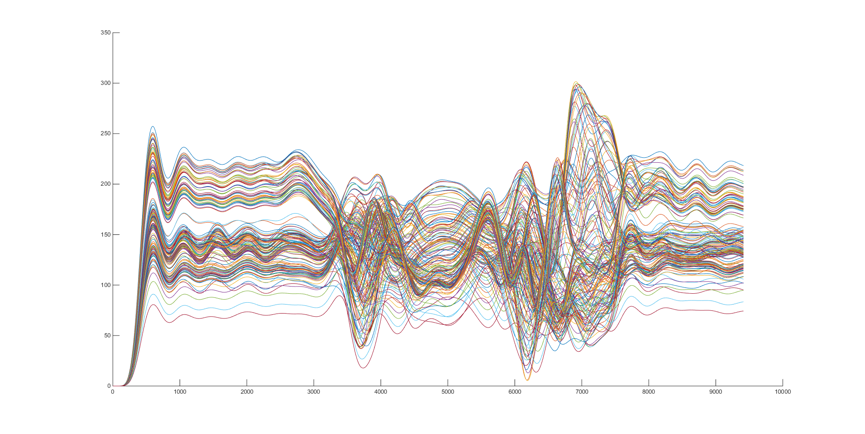
\includegraphics[width=4in]{corrfig_4}
  \caption[环境规律变化对子载波的影响]{环境出现规律变化时和同一天线有关的子载波开始变得相关}
  \label{fig:corrfig_4}
\end{figure}

\subsection{动作存在性检测模型}
手势识别的第一步即是检测是否有手势存在。如上文所述手势的存在与否对CSI的影响反映在两个方面:对CSI幅值的影响和对子载波间相关性的影响。因此我们通过结合这两个因素判断是否有手势存在。

\subsubsection{基于CSI幅值变化}
手势对CSI幅值的影响表现为:随着手势进入和离开信号传播主路径,CSI幅值会先后出现波谷和波峰。只需检测波谷和波峰的出现便可以感知到动作的存在。绘制CSI幅值随时间的变化图,通过人眼可以快速判断波谷波峰的存在,但对于计算机来说这种方法并不适用。一方面,需先将连续变化的波形转化为计算机更容易处理的方波。另一方面,即使不存在手势,CSI幅值也会有一定幅度的随机波动,这种波动会对判断结果产生干扰,算法需考虑抗干扰设计。具体算法设计如下:

\begin{compactenum}
\item 对原始CSI信号进行处理,去除毛刺。采用滑动窗口平均法,假设原始信号为$M \left( i \right)$,取窗口大小值$size_{window} = 300$,则处理过程如公式~\ref{equ:window_mean}所示。
\begin{equation}
\label{equ:window_mean}
{M_{mean}}\left( i \right) = mean\left\{ {\sum\limits_{k = i - size_{window} + 1}^i {M\left( k \right)} } \right\}
\end{equation}

\item 计算当前点${M_{mean}}\left( i \right)$相对于${M_{mean}}\left( i - size_{gap} \right)$的波动情况$\alpha \left( i \right)$。其计算方法如公式~\ref{equ:alpha}所示。
\begin{equation}
\label{equ:alpha}
\alpha \left( i \right) = \left\{ {\begin{array}{*{20}{c}}
{\begin{array}{*{20}{c}}
1&{,if\left( {\frac{{{M_{mean}}\left( i \right) - {M_{mean}}\left( {i - siz{e_{gap}}} \right)}}{{{M_{mean}}\left( {i - siz{e_{gap}}} \right)}} > \theta } \right)}
\end{array}}\\
{\begin{array}{*{20}{c}}
{ - 1}&{,if\left( {\frac{{{M_{mean}}\left( i \right) - {M_{mean}}\left( {i - siz{e_{gap}}} \right)}}{{{M_{mean}}\left( {i - siz{e_{gap}}} \right)}} < \theta } \right)}
\end{array}}\\
{\begin{array}{*{20}{c}}
0&{,otherwise}
\end{array}}
\end{array}} \right.
\end{equation}
公式~\ref{equ:alpha}中的$size_{gap}$和$\theta$需根据不同环境做相应调整,其中$size_{gap}$取值在300左右,$\theta$取值在0.2左右。

\item 当$\alpha \left( i \right)$出现$ - 1 \to 0 \to 1$的变化时,即表示出现了一个波谷。当$\alpha \left( i \right)$出现$1 \to 0 \to - 1$的变化时,即表示出现了一个波峰。

\item 出现波谷波峰的状态即认为可能有动作存在。
\end{compactenum}

将连续波形图转换为方波的结果如图~\ref{fig:MtoAlpha}所示。
\begin{figure}[htbp] % use float package if you want it here
  \centering
  \includegraphics[width=3in]{MtoAlpha}
  \caption{连续波形到方波的转换}
  \label{fig:MtoAlpha}
\end{figure}

\subsubsection{基于子载波间相关性变化}
利用子载波相关性指标检测动作是否存在的过程如下:
\begin{compactenum}
\item 滑动窗口计算子载波间相关性。
\item 对求得的相关性进行平滑处理。
\item 将平滑处理后的连续波形转化为方波,方法同对CSI的幅值的处理。
\item 当方波出现$1 \to 0 \to - 1$的变化时,即认为有动作出现。
\end{compactenum}

\subsection{动作数量检测模型}
动作数量的检测发生在动作存在性检测之后。首先确定动作的起始点和终止点,进而确定一段信号中包含的动作个数。当出现连续$size_{stable}$个采样点没有检测到波峰或波谷时,我们认为出现了一段稳定的信号。起始点发生在一段稳定信号后的第一个波动点回退若干采样点的位置,假设在一段稳定信号后检测到的第一个波谷或波峰发生在位置$i$,则动作的起始点大概在$i - size_{gap}$。终止点发生在一段稳定信号前的最后一个波动向后延迟若干采样点的位置。其中$size_{stable}$和$size_{gap}$的取值由手势参数有关,本文中分别取经验值3000和300。


\subsection{基于SVM的动作分类模型}
            
\subsubsection{SVM算法简介}

SVM(Supported Vector Machine)是机器学习中的一种常用算法,本质上一个二类分类器。假设训练集中有两类样本,如图~\ref{fig:svm}所示,我们的目的是寻找一个超平面(二维空间中对应为一条直线)将两类分开。这样当有一个新的样本出现是,我们就可以根据样本是在超平面的哪一边来判断样本属于哪一类。事实上,这样的超平面不唯一,如何从众多超平面中找出最优的一个便成了算法的重点。传统方法是定义一个损失函数,用最小二乘法求出一个局部最优值。而SVM的基本思想是让超平面最近的点离它尽可能远。图~\ref{fig:svm}中,两条虚线上的点即是离超平面最近的点,根据SVM算法的思想,求出的最优超平面即是图中所示的实线。

\begin{figure}[htbp] % use float package if you want it here
  \centering
  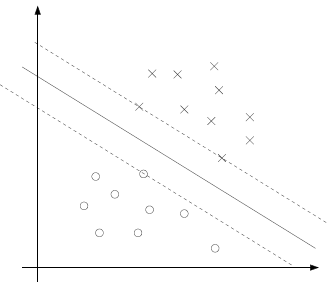
\includegraphics[width=3in]{svm}
  \caption{SVM算法分类思想}
  \label{fig:svm}
\end{figure}

\subsubsection{分类特征}
信号的分类特征大致包含两类,一类是几何特征,一类是统计特征。由于CSI变化具有一定的随机性,难以在不损失手势信息的情况下处理出完美平滑的曲线,因此其不易提取几何特征。本文使用统计特征作为SVM的输入。

传统统计类特征多使用均值,方差等统计量。本文首先基于这些基本特征进行了尝试。对于一段长度为$K$的CSI,将其分为20段,求出每段的均值、方差,组成40维特征向量,利用SVM分类。结果十分令人不满意。

考虑到手在运动过程中最直接影响的是CSI幅值,我们想到了将幅值分布作为分类的主要特征。三天线设备接收到的CSI中共包含$3 \times 3 \times 56$维数据,分别对应不同子载波,其中也包含了冗余及干扰信息。提取幅值分布前需先对CSI进行主成分分析(Principal components analysis,PCA)并降维。经实验,相比于对$3 \times 3 \times 56$维数据进行PCA,只取一根天线相关的$1 \times 3 \times 56$维数据进行PCA更有效。

提取出的幅值分布中除了包含手势信息外,还有环境信息。相对于动态的手势,环境信息对CSI的影响表现为静态形式,即无手势时,环境的影响也存在。因此只需将后一窗口的幅值分布与前一窗口的幅值分布做差即可消除环境的影响,只保留幅值的变化情况。

综上,特征向量的提取步骤如下:

\begin{compactenum}
\item 从$3 \times 3 \times 56$维CSI数据中提取出和接收端某一根天线有关的$1 \times 3 \times 56$维CSI数据。
\item 对提取的CSI数据进行主成分分析,并降维到56维。
\item 分别对每组数据分帧,并计算每一帧的幅值分布。
\item 对相邻帧的计算结果做差,消除环境影响,只保留幅值分布的变化信息。
\end{compactenum}

\section{性能评估}
本节将通过实验来评估本章中提出的算法性能。主要考虑算法对手势集中五个手势的兼容性以及识别正确率。评估实验共设计三组,对应三种不同的环境:不穿墙无障碍物,不穿墙有障碍物,穿墙。每组实验为每个手势采集20个样本,每个样本中包含两次重复的手势,此外每组实验中还会采集30个无任何手势的样本。

\subsection{存在性检测}
用本章提出的方法,对采集的样本进行测试,测试结果如表~\ref{table:exist_detection}所示,表中内容表示算法检测判定为存在动作的样本个数占该组样本总数的比。例如,表格第一行第一列中19/20,表示第一组数据中和手势a有关的样本共20个,其中算法正确检测出19个。

\begin{table}[htb]
  \centering
  \caption{动作存在性检测结果}
  \label{table:exist_detection}
  \begin{tabularx}{0.9\linewidth}{|X|X|X|X|}
  \hline
  &{\hei 第一组} &{\hei 第二组} &{\hei 第三组}  \\
  \hline
  {\hei 手势a} & 19/20 &  18/20 &  20/20  \\
  \hline
  {\hei 手势b} & 19/20 &  16/20 &  14/20  \\
  \hline
  {\hei 手势c} & 20/20 &  20/20 &  19/20  \\
  \hline
  {\hei 手势d} & 19/20 &  20/20 &  20/20  \\
  \hline
  {\hei 手势e} & 20/20 &  19/20 &  20/20  \\
  \hline
  {\hei 无手势} & 4/30 &  4/30 &  2/30  \\
  \hline
  \end{tabularx}
\end{table}
从表~\ref{table:exist_detection}记录的结果可以看出,算法对环境存在一定的鲁棒性,但是对手势的兼容性还需进一步提高。虽然较准确的检测出手势a、手势e,但对手势c、手势d的检测准确率低。

\subsection{数量检测}
数量检测的评估重点在于验证算法能否正确判断出样本中包含的手势数量。如上文所述,评估实验中没个样本包含两个手势,若算法判断为包含两个手势,即正确,否则即判断错误。具体的检测结果如表~\ref{table:num_detection}所示。表中每一行代表一种手势的检测结果,例如第一行表示,60个包含手势a的样本,算法检测认为56个样本中包含两个手势,3个样本中包含多个手势,1个样本中包含少于两个手势。

\begin{table}[htb]
  \centering
  \caption{动作数量检测结果}
  \label{table:num_detection}
  \begin{tabularx}{0.9\linewidth}{|X|X|X|X|}
  \hline
  检测出的手势个数&{\hei 0或1} &{\hei 2} &{\hei 3及以上}  \\
  \hline
  {\hei 手势a} & 1 &  56 &  3  \\
  \hline
  {\hei 手势b} & 9 &  49 &  2  \\
  \hline
  {\hei 手势c} & 1 &  51 &  8  \\
  \hline
  {\hei 手势d} & 4 &  55 &  1  \\
  \hline
  {\hei 手势e} & 1 &  58 &  1  \\
  \hline
  \end{tabularx}
\end{table}

\subsection{SVM分类性能}

本部分对SVM分类性能的评估共做了三组评测,分别是基于传统统计特征的分类,基于全部CSI幅值分布特征的分类和基于其中一根天线有关的CSI幅值分布特征的分类。

其中基于均值,方差做特征进行SVM分类分布的结果如表~\ref{table:svm:std}所示。表中每一行表示某手势样本的分类结果,每一列表示分到对应类的样本占该手势样本的比例。所以对角线上的值越高表示效果越好。

表~\ref{table:svm:std}表明,基于均值,方差的分类效果差,保持在30\%左右,只比随机分类高出10个百分点。
\begin{table}[htbp]
  \centering
  \caption{基于均值方差特征的分类结果}
  \label{table:svm:std}
  \begin{tabularx}{0.9\linewidth}{|X|X|X|X|X|X|}
  \hline
  &{\hei 手势a} &{\hei 手势b} &{\hei 手势c} &{\hei 手势d} &{\hei 手势e} \\
  \hline
  {\hei 手势a} & 31.25\% & 18.75\% & 21.88\% & 12.5\% & 15.63\% \\ 
  \hline
  {\hei 手势b} & 18.75\% & 31.25\% & 12.5\% & 34.38\% & 3.13\%  \\
  \hline
  {\hei 手势c} & 9.38\% & 18.75\% & 37.5\% & 15.63\% & 18.75\%  \\
  \hline
  {\hei 手势d} & 15.63\% & 28.13\% & 18.75\% & 28.13\% & 9.38\%  \\
  \hline
  {\hei 手势e} & 6.25\% & 6.25\% & 46.88\% & 18.75\% & 21.88\%  \\
  \hline
  \end{tabularx}
\end{table}

相比于均值方差特征,基于全部CSI幅值分布特征做分类效果会好很多,其分类结果如表~\ref{table:svm:hist1}所示。可以看出,分类的准确率有了质的提升。但还是无法令人满意。

\begin{table}[htbp]
  \centering
  \caption{基于全部CSI幅值分布特征的分类}
  \label{table:svm:hist1}
  \begin{tabularx}{0.9\linewidth}{|X|X|X|X|X|X|}
  \hline
  &{\hei 手势a} &{\hei 手势b} &{\hei 手势c} &{\hei 手势d} &{\hei 手势e} \\
  \hline
  {\hei 手势a} & 84.38\% & 3.13\% & 3.13\% & 9.38\% & 0\%   \\ 
  \hline
  {\hei 手势b} & 0\% & 93.75\% & 0\% & 0\% & 6.25\%  \\
  \hline
  {\hei 手势c} & 0\% & 12.5\% & 65.63\% & 12.5\% & 9.38\%  \\
  \hline
  {\hei 手势d} & 0\% & 6.25\% & 18.75\% & 71.88\% & 3.13\%  \\
  \hline
  {\hei 手势e} & 0\% & 15.63\% & 6.25\% & 0\% & 78.13\% \\
  \hline
  \end{tabularx}
\end{table}

当我们从全部CSI数据中抽取出和某一个天线有关的CSI,然后再从中提取幅值分布特征,其分类结果有了进一步盖上。具体如表~\ref{table:svm:hist2}所示。可以看到,表中前三个手势的分类准确率在90\%以上,即使表现很差的手势d和手势e,其分类准确率也可达80\%。

\begin{table}[htbp]
  \centering
  \caption{基于部分CSI幅值分布特征的分类}
  \label{table:svm:hist2}
  \begin{tabularx}{0.9\linewidth}{|X|X|X|X|X|X|}
  \hline
  &{\hei 手势a} &{\hei 手势b} &{\hei 手势c} &{\hei 手势d} &{\hei 手势e} \\
  \hline
  {\hei 手势a} & 96.88\% &  0\% &  3.13\% &  0\% &  0\% \\
  \hline
  {\hei 手势b} & 0\% &  96.88\% &  3.13\% &  0\% &  0\% \\
  \hline
  {\hei 手势c} & 3.13\% &  0\% &  93.75\% &  3.13\% &  0\% \\
  \hline
  {\hei 手势d} & 6.25\% &  9.38\% &  3.13\% &  81.25\% &  0\% \\
  \hline
  {\hei 手势e} & 6.25\% &  0\% &  12.5\% &  0\% &  81.25\% \\
  \hline
  \end{tabularx}
\end{table}

\section{本章小结}

本章详细介绍了一种基于Wi-Fi信号的手势感知技术。先从实际需求出发,引出手势感知的重要性。接着对比现有手势感知技术分析了基于Wi-Fi信号感知的优势及困难。然后介绍了基于Wi-Fi感知所用到的CSI数据的获取办法,并对CSI数据与环境的关系做了深入的分析。进一步介绍了手势感知手势感知中面临的手势存在性检测、手势起始点检测、和手势分类三个主要问题,并提出了相应解决方法。最后,本章对文中提出的方法做了性能评估。

% \chapter{基于 WiFi 的人体动作感知}
% \section{引言}
% \subsection{感知需求及存在的困难}
% 人体靠近检测

% 动作存在性检测

% 动作数量判断

% \section{已有的工作}
% 基于 RSSI
% 基于 视频
% 基于 红外
% 基于 加速传感器陀螺仪

% \section{基于 CSI 感知人体动作}

% \subsection{理论支持}

% \subsection{实验支持(相关性分析)}
% 正文内容
% \section{系统设计}

% \subsection{CSI 数据获取}
% \subsection{CSI 的预处理}
% 窗口均值 波形变换 滤波 主成分分析

% \subsection{利用 SVM 的动作分类}

% 特征选择及提取过程

% \section{性能评估}
% 正文内容
% \subsection{实验设计}
% \subsection{结果与分析}

% \section{本章小结}